%%%%%%%%%%%%%%%%%%%%%%%%%%%%%%%%%%%%%%%%%%%%%%%%%%%%%%%%%%%%%%
%%%%
%%%%  Project October
%%%%
%%%%%%%%%%%%%%%%%%%%%%%%%%%%%%%%%%%%%%%%%%%%%%%%%%%%%%%%%%%%%%
\documentclass[11pt,letterpaper]{article}
\usepackage[utf8]{inputenc}
\usepackage[letterpaper,includeheadfoot, top=0.5cm, bottom=3.0cm, right=2.0cm, left=2.0cm]{geometry}
\renewcommand{\familydefault}{\sfdefault}

\usepackage{graphicx}
\usepackage{color}
\usepackage{amsmath}
\usepackage{fancyhdr}
\usepackage{paralist}
\usepackage{hyperref}
\usepackage{subfig}
\usepackage{pdfpages}
\usepackage{amssymb}
\usepackage{url}
\usepackage{listings}

\usepackage{listings} %Code
\lstset{language=C, tabsize=4,framexleftmargin=5mm,breaklines=true}

\hypersetup{
    colorlinks,%
    citecolor=black,%
    filecolor=black,%
    linkcolor=black,%
    urlcolor=black
}

\begin{document}
%\begin{sf}

\newpage
\pagestyle{fancy}
\fancyhf{}
\fancyhead[L]{ 
\includegraphics[scale=0.3]{img/cwru-formal-logo-blue-no-tag.png} }
\vspace*{6cm}
\begin{center}
\Huge  {Project October}\\
\vspace{1cm}
\huge {Read news that you want to read}\\
\vspace{1cm}
\end{center}
%----------------- Names ------------------------
\vfill
\begin{flushright}
\begin{tabular}{ll}
Authors: & Tom Dooner, Mika Little, Brian Stack\\
Project: & Project October\\
Date: & \today
\end{tabular}
\end{flushright}

\newpage
\pagestyle{fancy}
\fancyhf{}

%\fancyhead[L]{\rightmark}
\fancyhead[L]{\small \rm \textit{\rightmark}}
\fancyhead[R]{\small \rm \textbf{\thepage}}


%\fancyfoot[L]{\small \rm \textit{Pie de página - Izquierda}}
%\fancyfoot[R]{\small \rm \textit{Pie de página - Derecha}}
%\fancyfoot[C]{\thepage} %Centro

\renewcommand{\sectionmark}[1]{\markright{\thesection.\ #1}}
\renewcommand{\headrulewidth}{0.5pt}
\renewcommand{\footrulewidth}{0.5pt}

% =============== Index ===============

\tableofcontents
\listoffigures

% =============== Section ===============
\newpage
\section{Abstract}

Longtime users of modern news aggregation services (such as Reddit, Slashdot, Digg, and Hacker News) report noticing a marked decrease in quality of discourse as the services gain mainstream attention.
This gradual but irreversible decline was noted as early as in the newsgroup era, when new college students would log in for the first time in September, causing an influx of new users and subsequently diluting discussion upon the sites which they joined.
As an example, after AOL opened newsgroups to the masses, the community standards continued to devolve, according to newsgroup veterans\cite{september}.
This gradual decline of content quality due to large numbers of new users came to be known as ``Eternal September'', being ``Eternal'' as the influx of new users was no longer restricted to September, but persisted through all months of the year.

October is a solution to this problem.
By providing users with an automatically-customized experience, we believe we can provide a large community to benefit from thoughtful discourse and interesting articles.
October will employ a technique to recommend news articles which, to our knowledge, is not currently applied on any other major news aggregators.
With custom recommendations for each user, we believe that a community can attain both size and quality.

\newpage

%----Everything else----%

\section{Project October: Hybrid Recommender System}

Due to the ever-growing amount of information available online, the need for a highly developed personalization and filtering system is growing significantly.
Recommender systems constitute a specific type of information filtering that
attempt to present items according the interests expressed by a user.
Most web recommenders are employed for e-commerce applications or customer
adapted websites, which assist users in decision making by providing
personalized information, but the same techniques that
suggest related items on e-commerce websites can recommend news articles to users as well.
We believe Project October is the first attempt to apply recommendation techniques to social news aggregation.

\subsection{Background}
It is our hypothesis that the recommendation of news sources will provide a scalable community experience that can be tailored to each person's interests.
Providing an automatic, customized, recommendation of articles will prevent the community from being diluted by new users and thus prevent the Eternal September phenomenon.
Each user will have their own viewing environment curated for them, with different mindsets and preferences forming their own communities in which like-minded individuals can partake in discussion, eliminating the cross-contamination of user bases.  

This proposal discusses an implementation of a hybrid collaborative and content-based filtering approach for a web-based recommender system (``October'').
In particular, we will be linking various news sources and user submitted sources.
The resulting network of user-item relations and associated content features is converted into a unified mathematical model, which is applicable to our underlying neighbor-based prediction algorithm.
By means of various experiments, we demonstrate the influence of supplementary users as well as item features on the prediction accuracy of October, our proposed hybrid recommender. In order to decrease system runtime and to reveal latent user and item relations, we factorize our hybrid model via singular value decomposition (SVD).

For the development and evaluation of our proposed hybrid recommender system, we make use of various news outlets and user recommendations, importing them into a graph database.
Both corpora are joined in a unified mathematical model, which describes the complex network of interdependencies.

\subsection{Intended Audience}
We intend Project October to be open to the public.
At launch, we expect the user base to be somewhat technical in nature, being some of the Internet's power users.

\subsection{Progress}
% Fill in with details of our progress -- how far we have come and where we
% will go from here

\subsection{This Report}
% First we will describe the two separate components of October -- the frontend
% and then the backend. Then we will describe the API which ties them together.
% Then, we will discuss *how* we built October, including the requirements and
% the project management. etc.

\section{Application}
\subsection{Frontend}
The frontend will be a standard social news aggregator.
Upon going to the homepage, new and logged-out users will be presented with a splash page that describes the nature of Project October and offers a registration link.
Users can register for the application by selecting a username and password.

When logged in, users will be presented with their personalized content.
The design is modelled after the front page of a newspaper -- articles that are evaluated to be more interesting to a user will be placed in more prominent positions while articles that are deemed less relevant to the user's interest will fill the side columns, be located further down the page, and occupy less space.
Users will be able to click on the headline (or associated image, if existent) to be taken to the original news source.

Each news article will feature a link to view the associated comments as well as an icon (located in the corner of the article text/image) displaying the credibility (``cred'') a given article possesses.
This is analogous to upvoting in Reddit, except that giving an article cred on October will inform the recommendation engine of your individual preference, rather than directly impacting the weighting of an article by a predefined formula. Therefore, cred serves two purposes: 1. To inform other users of the quality of the article and 2. To inform the recommender system of the user's interests.

Users will be able to click a link on the homepage which takes them to an article submission form.
The submission form will request a URL and a headline for that news story.
Upon entering the URL, the news story will be scraped in the background using a web scraping tool which will attempt to extract properties about the page automatically -- relying upon the <meta> tags and heuristics to determine the article's body text.

\subsection{Backend}
The backend will contain a recommender system, which will recommend articles for users with the following technique.
When an article is submitted from the frontend (via the API -- see Section \ref{sec:api}), we will peform TF/IDF\cite{tfidf} on the full body text returned by the scraper.
The weighted terms returned by TF/IDF will be stored in a document database with a custom-maintained inverted index of the terms to which articles contain them.
This will allow efficient access of articles about arbitrary terms.

When a user upvotes, downvotes, reads, or comments upon an article, the user's document will be modified to reflect that the user either cares more (in case of upvotes, comments, or reads) or cares less (in case of downvotes) about the terms associated with that article.
When the frontend requests more articles via the API for that user at a later time, the new weights will be used, resulting in a different, more-tailored selection of news articles.

The backend and the frontend will share access to the frontend database, which will contain all persistent information about articles such as their headline, image thumbnail URL, and other associated metadata.
The backend will have read-only access to the frontend database.
The backend will have exclusive control of a document database which tracks information about users and article terms.

\subsection{Frontend/Backend API}
\label{sec:api}
October will employ an API to promote separation between the frontend and the backend recommender system.
This will provide a clear interface and facilitate easy simultaneous development of both parts of October.

To implement the API, we will use Apache Thrift, an Interface Description Language\cite{thrift}.
The essence of the API is simple, featuring primarily two types of calls:
\begin{description}
\item[Give $n$ recommendations for user $u$]
This is the main output from the backend, returning recommended news stories or comments for a given user.
Ancillary parameters will be added to this to facilitate the frontend placement of articles, e.g. the recommendation confidence and individual article weightings.
\item[User $u$ took action $n$]
This is the main input to the backend, allowing it to adjust recommendations according to user action.
The parameters to this API call can be of many types. For example, "User commented on article \#$n$", "User gave cred to comment \#$n$", and "User visited link \#$n$" are all valid parameters for this API call.
\end{description}

These two calls manifest themselves in Thrift with a few simple object
definitions and an interface.  The abbreviated version \texttt{0.1.0} is
attached as Appendix~\ref{app:thrift}.

\section{Software Design}
% This section will describe the progress towards the usual software design information, with likely components on
% - Application Software Requirements
% - Application Software Specifications
% - Software Architecture (i.e., client - server architecture; three - tiered design, etc.)
% - Design Document

\subsection{Intended Audience}
We intend October to be open to the public.
Although the user base is currently somewhat technical in nature, October supports the registration of any internet user.

\subsection{Homepage Requirements}
The are two cases for the homepage: logged in users and logged out users.

Logged out users arrive at the homepage and are presented with a splash page containing a description of October's features.
There is a registration link so that interested users can register for their own account.

Logged in users should, upon landing on the homepage, be quickly presented with a display of news articles.
The display will be pictures (when available) along with the headlines for each article.
Each article should be accompanied with links to positively influence the article's recommendation rank, to negatively influence the article, and to comment on the article.

\subsection{User Creation/Login/Display Requirements}
Internet travelers should be able to create accounts on October easily by providing minimal information -- simply their desired username, their email, and a password.
After creating a user, an email should be sent to the user welcoming them to October.

When a user first uses October, the backend recommender won't know anything about that user's interests.
Thus, users should be shown various sample topics and the ability to manually input keywords until the recommender is confident enough in their browsing habits to make recommendations.

Every mention of a user's name (i.e. the credit for who posted an article or comment) should be a link to a user profile page. More detail about the user profile page is given in Section \ref{sec:profilepage}.

\subsection{User Profile Page Requirements}
\label{sec:profilepage}
Each user has a profile page containing information related to that user.
The profile page contains a list of comments that the user has made on posts and a list of articles the user has posted.
All information on this page is public, as it is merely a summary of content available elsewhere on the public website.

\subsection{User Profile Edit Page Requirements}
In contrast to the profile page, which is a summary of a user's public activity, the profile edit page allows a logged in user to edit their own information.
Settings such as their email address and password can be changed here.

The other significant part of the user profile edit page is a section which shows the user their own recommendation settings.
This shows up in the format of a list of keywords that the backend has ascribed to that user.
The user can remove keywords that they do not wish to be associated with.

Furthermore, there should be a field where a user can submit additional keywords they wish to see more news from.
The user will be associated with the keyword when they submit the form.

\subsection{Article Posting Requirements}
Logged in users should be able to click a prominent link on the homepage to submit a story.
The submit story page will ask for the link to the desired story, and automatically show the results of scraping that story's contents (see Section \ref{sec:scraping} for more about scraping).
If the post looks good to the user, he or she can click a ``Post!'' button, which will persist the news story in all appropriate databases.

\subsection{Article Page Requirements}
The article display page is a page dedicated to a posted news article. Every news article has an associated article page.
The intent of the article page is to facilitate sharing of opinions around the posted news story through comments.

A user arriving on an article's page arrives at a page which contains the title of the news article along with a threaded comment list.
Users may leave comments as children of other comments, and thus may engage in a lively discussion.

\subsection{Frontend $\leftrightarrow$ Backend API Requirements}
Since the frontend and backend are divided with a Service Oriented Architecture (with Apache Thrift bridging the gap\footnote{See Section \ref{sec:api} for more about Thrift}), there must be an API between them.

The API should be as simple as possible to maintain the functionality of October. This is not a public API, so it needs to be robust to volume but we do not need to implement API endpoints for the functionality mentioned elsewhere in the requirements.

The API is defined in a Thrift definitions file in the project-october-api repository on GitHub\cite{project-october-api}.

\subsection{Web Scraping Requirements}
\label{sec:scraping}
When a user submits a link to a news article, October needs to know three more things about each article than just its URL: 1) the title of the article, 2) any associated images, and 3) all the main keywords from the article.
We will employ the pismo library\cite{pismo} which, given the URL to a webpage, performs extractions of all these things automatically.

The pismo library is used to return all these things to the frontend, which then allows users to customize the image selection, keywords, and the title if necessary before the article is submitted.

\subsection{Backend Requirements} % Expand into multiple sections?
The backend is a recommender black-box which provides suggestions via an API to the frontend.
The actual implementation of the recommendation service is arbitrary, only that it implements the services of the API effectively.
For more about the implementation of the backend, consult Section \ref{sec:backend-implementation}.

\section{Project Management--Administrative Details}
% Design/update your Gantt chart to show any changes in milestones, timetable,
% or responsibility (especially if there are multiple team members). Be sure to
% properly indicate who is actually performing each task and the degree of
% completion of each task.  Describe how well the project management plan is
% working. Were there unforeseen problems with any of the tasks that you ha ve
% had to work around? Are there delays in obtaining parts or software?  Were
% major changes to the management plan or back - up plans requ ired and
% implemented? What work - arounds were necessary to keep the project on
% schedule?  It is very important that you des cribe any changes in the project
% plan since the proposal and the reasons for them.  Finally, use your
% management plan to carefully think about what can be realistically done by
% your 3 team between now and the end of the semester.

\begin{figure}
\centering
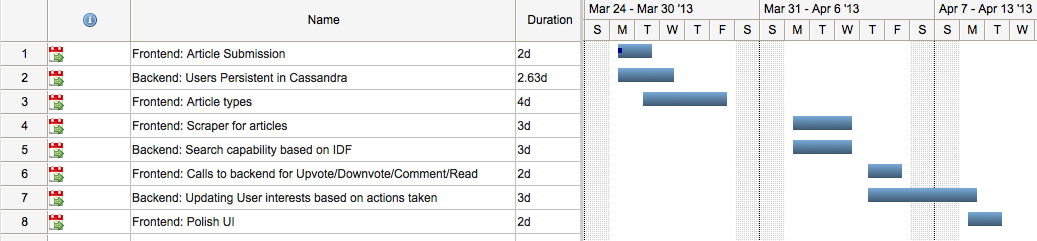
\includegraphics[scale=0.45]{img/octoborg-gantt.png}
\caption{Project October Gantt Chart}
\label{fig:gantt}
\end{figure}

We have split the team into two parts, frontend and backend.
With respect to the frontend, Tom and Mika have worked on the development and design respectively.
The biggest difficulty here is to determine how to represent the news in such a way that the user will be inclined to continue using the service.
As for the backend, Brian has been tasked with creating both the service architecture and the recommender engine.
This includes the implementation of our backend's TF-IDF algorithm and the Scala connector to the Thrift API and Mongo that computes recommendations.

\subsection{Release v1.0}
In Project Report 2, we promised a fully-functional beta by ``early to mid-April''.
On April 15th, we released the beta to the CWRU community, and it has been met with a warm reception.

\section{User Interface}
The user interface for the homepage and other pages will surely evolve over time.

The homepage is an especially crucial interface to get right. We mimic a newspaper feel with articles staggered in a rough column grid.
This allows readers to be presented with many recommendations of different weights simultaneously in a manner in which they are accustomed to. 
Cred will be handled by placing two links (upvote and downvote) into the article area, along with the link to the comments next to it. 
The search bar, along with a 'Submit Article' button, and Profile drop-down menu will be located at the top of the site. The latter will include options such as "view posts", "Profile Edit", "New Messages/Comments" and "Logout".
The comments on each article are handled in a nested fashion, with each comment and reply having their own attributed cred value. 
% TODO: Make sure we change this line/section as we go through the project:
A pre-Alpha screenshot of the homepage is attached in figure \ref{fig:homepage}.

\begin{figure}
\centering
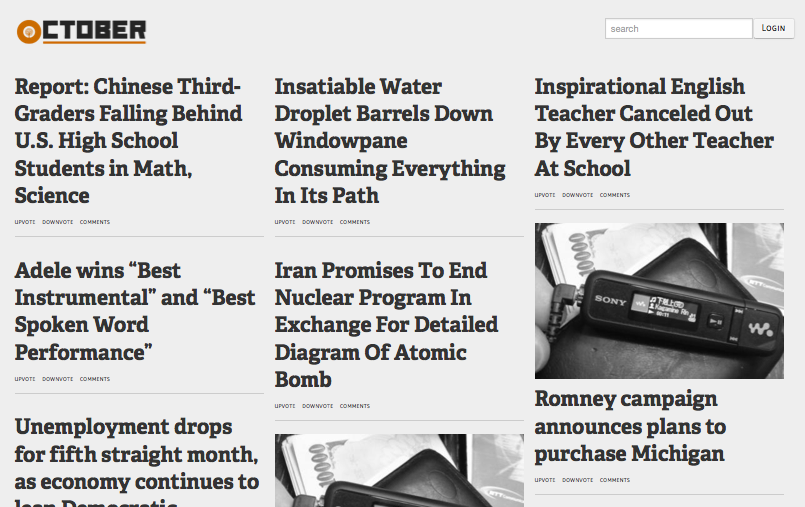
\includegraphics[scale=0.35]{img/homepage.png}
\caption{Project October Homepage, pre-Alpha (Headlines courtesy The Onion)}
\label{fig:homepage}
\end{figure}

The user interface for other pages will be in the same general content area, however there are no further screenshots to share at this time.

\section{Testing \& Evaluation}
Testing and evaluation will be performed as we progress through the project. Currently, only very minimal testing is implemented.

\section{Project Progress}
% This section should summarize the progress (or the lack of it) so far, and
% address any issues that have arisen recently.
The project is progressing satisfactorily.
We are attempting to follow Agile Design Patterns, and we have been effective at meeting for short periods frequently.
On the frontend, we have completed the user creation + login processes, mocked up the homepage, and connected the Thrift library.
On the backend, we have implemented the API so it responds to requests from the frontend. The recommendation engine is still in-progress.
We remain committed to maintaining team communication via scrum and continue working.

\subsection{Discussions \& Conclusions}
% These conclusions are not really conclusions since your project is not yet
% finished. In this section you should discuss whether the project is on
% schedule for completion at the end of the semester. Are there major problems
% which require a reevaluation of the project results? If not, what is the new
% schedule and what do you plan to have done by the end of the semester? You
% can also comment on things which have worked better than expected or proved
% easier to solve.
Overall, the project is still on schedule. We still intend to complete a fully-featured product on-time.

\section{Lessons Learned}
\newpage

%The lessons we've gleaned through development. If you've had any personal %revelations, visions, or epiphanies, please share below. 
Throughout the development of October, we gained insight as how to properly design and create a product that will be used by many. 
Foremost among lessons learned, is that agile development ended up not being suitable for our work agenda. 
It required a certain rigidness in our schedules that we could not maintain. 
Instead, periodic scrum meetings sufficed for communicating progress and sharing ideas. 

Alongside the ineffectiveness of agile development in a college setting, an important lesson was learned when October was first released to the public in early April. 
Based on user feedback, we learned that October was, in fact, a viable web service, and we have had moderate user retention. 
We have enjoyed working on this, and we hope to continue refining it after the class is over. 
We will be keeping in contact with users to build upon October, enhancing the service and hopefully increasing user retention.
 
 

\section{Appendix}

% ============= References ==============
\newpage
\newpage
\begin{thebibliography}{6}
  \bibitem{september} \url{http://en.wikipedia.org/wiki/Eternal\_September}
  \bibitem{thrift} \url{http://en.wikipedia.org/wiki/Apache\_Thrift}
  \bibitem{tfidf} \url{http://en.wikipedia.org/wiki/Tf-idf}
  \bibitem{pismo} \url{https://github.com/peterc/pismo}
\end{thebibliography}

% ============= Database Schematic ==============
\newpage
\appendix
\section{Thrift API Definition}
\label{app:thrift}
\begin{verbatim}
#
# Structs
#

/** A single post with its calculated weight.
 * @param post_id, the unique id of a post.
 * @param weight, the "importance" of the post to the querying user [0,1].
 */
struct Post {
    1: required i64 post_id,
    2: optional double weight,
}

/** A list of posts along with a confidence for the accuracy of the list.
 * @param confidence, the confidence in the results.
 * @param posts, a list of Posts.
 */
struct PostList {
    1: optional double confidence,
    2: required list<Post> posts,
}

/** The types of actions that can be performed in a triple (subject, verb, object) */
enum Action {
    READ,
    VOTE_UP,
    VOTE_DOWN,
    VOTE_NEGATE,
    POST,
    COMMENT,
    REPORT,
    TAG
}

#
# Exceptions
#

/** The queried object does not exist. */
exception NotFoundException {
}

/** There was an error processing the request */
exception EngineException {
    1: required string why,
}

/** Request took too long to process */
exception TimeoutException {
}

#
# Service
#

service Recommender {

    /** Test for connectivity */
    string ping() throws (1: TimeoutException te),

    /** Request a list of posts that are most appropriate for a user
     * @param user_id, the user that the posts are being requested for
     */
    PostList recPosts(1: required i64 user_id) throws (1: NotFoundException nfe, 2: EngineException ee, 3: TimeoutException te),

    /** Alert the recommender that a user has actioned a post
     * @param user_id, the user that performed the action
     * @param verb, the action taken (this is from the Action enum)
     * @param post_id, the post that the action is being performed on
     */
    void user_v_post(1: required i64 user_id, 2: required Action verb, 3: required i64 post_id) throws (1: NotFoundException nfe),

    /** Alert the recommender that a user has actioned a comment
     * @param user_id, the user that performed the action
     * @param verb, the action taken (this is from the Action enum)
     * @param comment_id, the comment that the action is being performed on
     */
    void user_v_comment(1: required i64 user_id, 2: required Action verb, 3: required i64 comment_id) throws (1: NotFoundException nfe),
}
\end{verbatim}

\section{Database Design}
\subsection{Frontend Database}
\begin{figure}
\centering
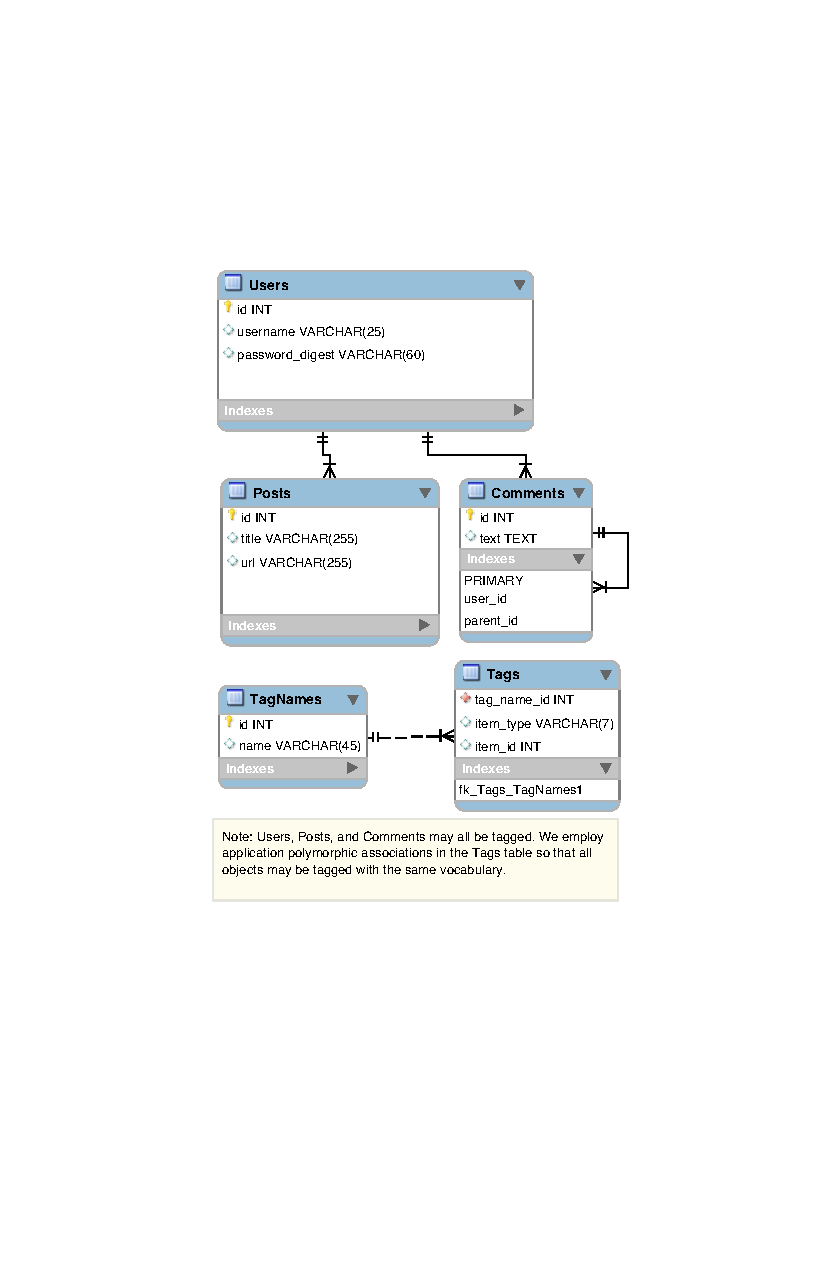
\includegraphics{db_diagram.pdf}
\caption{Frontend Database Relational Diagram}
\label{fig:database}
\end{figure}
Please see Figure \ref{fig:database}.
\subsection{Backend Database}

\section{User Manual}

\section{Programmers Manual}
% ============= FIN ==============

\end{document}
